\RequirePackage{fix-cm}
\documentclass[preprint,review,12pt]{elsarticle}

\usepackage[T1]{fontenc}
\usepackage[utf8]{inputenc}
\usepackage{amsmath,amssymb,amsthm,mathtools}
\usepackage{graphicx}
\usepackage{booktabs}
\usepackage{array}
\usepackage{tabularx}
\usepackage{enumitem}
\usepackage{float}
\usepackage{xcolor}
\usepackage{xurl}
\usepackage{microtype}
\usepackage[hidelinks]{hyperref}

\definecolor{pendingred}{RGB}{166,24,24}
\newcommand{\AuthorPending}[1]{\textcolor{pendingred}{[AUTHOR INPUT REQUIRED: #1]}}
\newcommand{\Acomp}{\mathcal{A}_{\mathrm{comp}}}
\newcommand{\Arect}{\mathcal{A}_{\mathrm{rect}}}
\newcommand{\Hlib}{\mathcal{H}}
\newcommand{\TV}{\operatorname{TV}}
\newtheorem{proposition}{Proposition}

\biboptions{numbers,sort&compress}
\setlength{\bibsep}{0pt plus 0.3ex}
\setlength{\emergencystretch}{2em}
\journal{Pattern Recognition}

\begin{document}
\begin{frontmatter}

\title{Certified Minimax-Regret Ranker Selection under Compatible Positive--Unlabeled Mixture Constraints}

\author[aff1]{Jihao Li\corref{cor1}}
\cortext[cor1]{Corresponding author. \AuthorPending{email address}}
\address[aff1]{Independent Researcher, Shenzhen, Guangdong, China.
\AuthorPending{complete postal address}}

\begin{abstract}
Selecting an already trained ranker from positive--unlabeled (PU) data requires
joint reasoning about an unknown positive-class prior and an unknown
positive-conditional distribution: these quantities cannot vary independently
because together they must generate the observed query distribution. Generic
minimax-regret, PU-shift, and total-variation (TV) methods address model
selection, distribution shift, or class-prior uncertainty, but a Cartesian
product of a TV ball and a prior interval discards this mixture compatibility.
We introduce MC-TV-PU, which retains coordinate-wise mixture constraints on a
finite query space, defines minimax regret over a frozen ranker library using a
single shared comparator, and returns set-valued selections through a strict
rational-enclosure oracle. A four-point construction proves analytically that
the compatible set and a matched rectangular relaxation with the same feasible
prior upper bound can select different rankers. The terminal run configuration
records a frozen empirical protocol with 15 rankers whose score partitions have
verified target-drug scaffold test-fold assignments, two source-anchor centers,
12 TV radii, and selector-anchor source cross-fitting.

The terminal selector reduced the 15-ranker library in all 24 center--radius
cells. However, source cross-fitting over 208 drugs, 563 evaluable episodes,
and 6,408 held-out records produced no cell whose average-precision (AP) point
difference was nonnegative against both prespecified baselines, and no
simultaneous AP lower bound was positive against both. The frozen practical
gate therefore failed. We retain this as a boundary result: the compatible
formulation is decision-nonredundant and exactly solvable, but conditional
cross-source practical value and an empirical mechanism advantage were not
established for this frozen library.
\end{abstract}

\begin{keyword}
positive--unlabeled learning \sep distributionally robust optimization \sep
minimax regret \sep ranker selection \sep drug--non-coding-RNA association prediction
\end{keyword}

\end{frontmatter}

\section{Introduction}

Drug--non-coding-RNA association databases record only a subset of reported
positive associations. An unrecorded drug--RNA pair may be an undiscovered
association or a true non-association. Model development commonly produces a
fixed collection of rankers and selects one by a validation metric. When
validation positives originate from different publications, experimental
systems, and study preferences, the empirical positive distribution is neither
the deployment query distribution nor an object that can be adjusted
independently of the unknown positive-class prior.

Let the finite RNA query design be \(Q\), the latent positive-conditional
distribution be \(p\), and the positive-class prior be \(\pi\). Every admissible
PU world must satisfy the coordinate-wise mixture constraint
\(\pi p_i\leq Q_i\). Placing \(p\) in a TV ball and \(\pi\) in an independent
interval creates a rectangular ambiguity set containing combinations that
cannot jointly produce \(Q\). Such a relaxation can do more than enlarge a
risk bound: it can reverse the final action selected from a finite model
library.

We therefore study a deliberately narrow and falsifiable decision problem. We
do not train a new representation model. Given a frozen ranker library, a fixed
query design, and source-anchor centers, we ask how to make an auditable robust
selection under uncertainty in both the positive prior and the
positive-conditional distribution. The decision criterion is a directed rank
loss difference under a compatible PU ambiguity set, macro-averaged over drugs
and maximized against one comparator shared across those drugs.

Our contributions are:

\begin{enumerate}[leftmargin=*,label=(\arabic*)]
  \item \textbf{A compatible decision formulation.} We preserve the
  coordinate-wise coupling between \(\pi\) and \(p\) and formulate frozen-library
  selection as shared-comparator minimax regret, rather than allowing a
  different worst-case comparator for every drug.
  \item \textbf{Certified computation and non-redundancy.} For rational plug-in
  inputs, we provide a strict enclosure oracle. A closed-form four-point
  instance gives a decision reversal between the compatible ambiguity set and
  a matched rectangular relaxation that uses the same feasible upper bound on
  \(\pi\).
  \item \textbf{A frozen boundary test.} The terminal configuration records the
  full sensitivity path, matched-rule ablations, and selector-anchor source
  cross-fitting over 15 rankers with verified target-drug scaffold test-fold
  assignments under the status
  \texttt{FROZEN\_BEFORE\_SELECTOR\_RESULTS}. Average precision
  (AP) is the primary endpoint and AUC is restricted to a loss-alignment
  diagnostic. The selector narrowed the library, but the cross-source AP gate
  failed; the complete result is therefore retained as an identification and
  practical-value boundary rather than promoted to a mechanism claim.
\end{enumerate}

The scope is equally important. We do not claim that the underlying models
were trained with publication-level isolation, that database zeroes are true
negatives, that \(Q\) is a natural biological population, that a chosen TV
radius has population coverage, that MC-TV-PU theoretically optimizes AP, or
that the method extrapolates to unseen chemical scaffolds. Because the frozen
empirical gate failed, we make no claim of cross-source practical selection
value, including within the studied chemical space.

Figure~\ref{fig:overview} summarizes the decision and validation pipeline.

\begin{figure}[t]
  \centering
  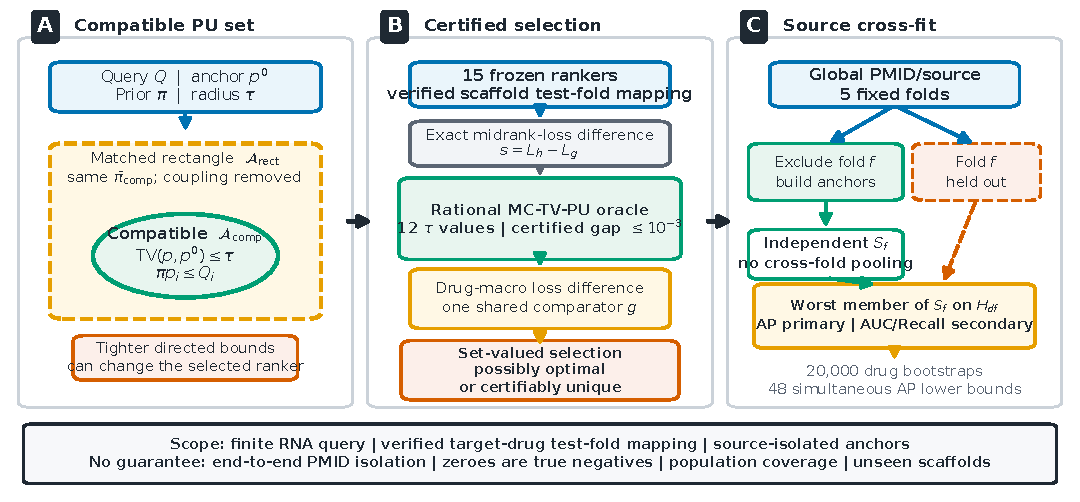
\includegraphics[width=0.98\linewidth]{figures/fig_mc_tv_pu_overview.pdf}
  \caption{MC-TV-PU decision and validation pipeline. For each drug (d), the
  observed query design \(Q_d\), source-anchor center \(p_d^0\), class prior
  \(\pi\), and positive-conditional distribution \(p_d\) define the compatible
  set through a TV constraint and coordinate caps
  \(\pi p_d(i)\leq Q_d(i)\). Exact directed loss-difference enclosures are
  aggregated across drugs and maximized over one shared comparator. The
  selector returns the possibly-optimal set; it does not break unresolved
  interval ties. Source cross-fitting reconstructs every fold-specific anchor
  center without that fold before evaluating newly recorded positives. AP uses
  a simultaneous lower band for the primary success gate; AUC and Recall use
  ordinary paired-bootstrap intervals and cannot rescue a failed AP gate. The
  matched rectangle uses the same feasible prior upper bound but deletes the
  coordinate-wise coupling.}
  \label{fig:overview}
\end{figure}

\section{Related Work and Novelty Boundary}

\paragraph{Minimax regret under distribution shift.}
Minimax regret and shared-comparator robust selection have direct antecedents,
including the general distribution-shift formulation of Agarwal and Zhang
\citep{agarwal2022minimax}. We do not claim these components in isolation. Our
delta is the decision problem induced by PU mixture compatibility, with an
unknown prior and a TV-perturbed positive distribution retained in the same
coordinate-wise constraint system.

Label-efficient comparison of frozen candidates is also not new in itself.
In a fixed finite evaluation pool, Kuboyama
\citep{kuboyama2026labelsdoesmodelchoice}
uses the fact that one queried label is shared by every candidate to construct
coupled label-completion certificates that are no looser than separately
computed candidate-risk completion intervals. That work targets selective
prediction and AUGRC under unrestricted completions of unread binary labels;
it does not encode a PU observation mechanism, an unknown drug-specific class
prior, or the coupled mixture and shifted-positive ambiguity studied here.

\paragraph{Positive--unlabeled distribution shift.}
Arbitrary positive shift has been studied by Hammoudeh and Lowd
\citep{hammoudeh2020arbitrary}, and labeling-mechanism identification under an
unknown class prior by He et al. \citep{he2026labeling}. These works preclude
claims that PU distribution shift,
unknown priors, or labeling mechanisms are new. We claim only the residual
decision-layer combination: compatible mixture coupling on a finite query
design, shared-comparator regret over a frozen ranker library, and a rational
enclosure oracle.

Importance-weighted PU adaptation provides another direct boundary. Kumagai
et al. \citep{pmlr-v258-kumagai25a} use positive and unlabeled samples from both source
and target distributions, assume both class priors known in the main
formulation, and alternate importance-weight estimation with classifier-risk
minimization. S-PUNA \citep{gabetni2026spuna} instead trains a covariate-shift
detector through bidirectional neighborhood pseudo-labeling, a spectral-entropy
stopping rule, and classifier distillation. Its total-variation term is the
balanced-prior, zero--one Bayes-risk identity, not a TV ambiguity radius.
Neither work poses a minimax-regret decision over a finite frozen candidate
set. We cite S-PUNA for this problem-and-algorithm boundary only, not as support
for a general entropy-monotonicity guarantee.

Table~\ref{tab:audited-neighbors} makes the residual boundary explicit. Each
row states the audited paper's own decision object and information structure;
the table is not an exhaustive absence claim over the literature.

\begin{table}[t]
\centering
\caption{Audited direct-neighbor boundary. ``Known priors'' refers to the main
paper formulation, even when external prior estimators are discussed.}
\label{tab:audited-neighbors}
\scriptsize
\setlength{\tabcolsep}{3pt}
\renewcommand{\arraystretch}{1.12}
\begin{tabularx}{\linewidth}{>{\raggedright\arraybackslash}p{0.17\linewidth}
  >{\raggedright\arraybackslash}p{0.20\linewidth}
  >{\raggedright\arraybackslash}p{0.31\linewidth}X}
\toprule
Work & Decision object & Shift/prior information & Output or guarantee \\
\midrule
Agarwal and Zhang \citep{agarwal2022minimax} & Model/function selection & Importance-weighted distribution family & Generic minimax-regret objective and statistical guarantees \\
Hammoudeh and Lowd \citep{hammoudeh2020arbitrary} & Newly trained classifier & Source/target unlabeled sets; stable negative conditional; known or estimated priors & Risk-consistent arbitrary-positive-shift learners \\
Kumagai et al. \citep{pmlr-v258-kumagai25a} & Newly trained classifier & Positive and unlabeled samples in both domains; known priors in the main formulation & Alternating importance-weight and risk minimization \\
He et al. \citep{he2026labeling} & Labeling-mechanism diagnostic & Positive and unlabeled observations with unknown prior & Global test of SCAR versus SAR \\
Gabetni et al. \citep{gabetni2026spuna} & Newly trained shift detector & Positive-domain sample and mixed pool; balanced-prior TV identity & Bidirectional pseudo-labeling and classifier distillation \\
Kuboyama \citep{kuboyama2026labelsdoesmodelchoice} & Frozen finite candidates & Shared unread labels in a fixed evaluation pool & Coupled label-completion certificates \\
MC-TV-PU (this work) & Frozen finite rankers & Fixed query design; unknown prior and shifted positive conditional jointly compatible with the observed mixture & Set-valued exact minimax-regret enclosure \\
\bottomrule
\end{tabularx}
\end{table}

\paragraph{Pairwise ranking and macro aggregation.}
BPR constructs observed--unobserved pairs from positive implicit feedback and
optimizes a pairwise ranking objective, while explicitly treating unobserved
items as a mixture of missing values and possible negative feedback rather
than confirmed negatives \citep{rendle2009bpr}. In fully labelled multi-label
learning, Wu et al. \citep{pmlr-v202-wu23l} define Macro-AUC as the equal-weight average
of label-wise bipartite-ranking AUCs and study label-wise imbalance and
reweighted losses. These works motivate, respectively, the pairwise loss and
macro aggregation used here. Neither identifies hidden positives under a PU
observation process or estimates an unknown drug-specific class prior.

\paragraph{Molecular and interaction generalization protocols.}
MoleculeNet groups molecules by two-dimensional Bemis--Murcko scaffolds and
uses scaffold splitting as a stronger structural-generalization test than
random splitting \citep{wu2018moleculenet}. DrugBAN further shows that a
drug-identity holdout can leave highly similar molecules across training and
test sets, and therefore evaluates an additional similarity-clustered
cross-domain split \citep{bai2023drugban}; that clustering is not equivalent
to Bemis--Murcko isolation. C2P2 transfers chemical--chemical and
protein--protein interaction knowledge to affinity prediction under unseen-
drug or unseen-target entity splits, but does not evaluate both entities
unseen or scaffold-disjoint extrapolation \citep{nguyen2022coldstartdta}.
Together these studies separate entity novelty, structural isolation, and
auxiliary-knowledge transfer. They motivate our evaluation boundary but do not
establish that MC-TV-PU generalizes to unseen scaffolds.

\paragraph{Drug--ncRNA ranking.}
The frozen rankers and data originate from the ncRD-LG study
\citep{xie2026ncrdlg}; MC-TV-PU is a post-training selection procedure and not a
new encoder or graph learner. Its evaluation therefore concerns conditional
selection within the existing chemical space, not generalization to unseen
scaffolds.

Task-specific predictors also cover regimes that we do not claim as new.
sChemNET learns from positive and unlabeled molecule--miRNA pairs and reports
chemically dissimilar evaluation subsets defined by a Tanimoto-similarity
threshold, rather than a documented Bemis--Murcko scaffold-disjoint split
\citep{galeano2024schemnet}. RAHGL-MDR reports entity cold-start and
full-candidate rankings; in its drug-cold MAP comparison, the reported
degree/popularity baseline exceeds the full graph model
\citep{elbashir2026rahgl}. HMVCC reports drug-level cold-start and
human-to-nonhuman transfer, while its reviewed protocol does not document
Bemis--Murcko isolation or drug-macro full-candidate AP
\citep{ma2027hmvcc}. Thus our contribution is neither a new encoder nor the
first cold-start evaluation. It is the decision-layer selection problem above,
and the failed source-crossfit gate does not establish superiority over these
predictors.

Adjacent RNA--small-molecule work further separates representation advances
from the decision problem studied here. RNAincoder provides reusable RNA and
compound descriptor encodings for multiple downstream interaction tasks
\citep{wang2023rnaincoder}. RNAmigos learns local RNA-pocket graphs for ligand
preference ranking, and RNAmigos2 extends structure-based virtual screening
with pocket-cluster isolation and synthetic augmentation
\citep{oliver2020rnamigos,carvajalpatino2025rnamigos2}. RSAPred studies binding-
affinity regression with external validation, whereas RNAsmol reports random,
cold-RNA, cold-small-molecule, and double-cold interaction-scoring conditions
\citep{krishnan2024rsapred,ma2025rnasmol}. MolVisGNN combines one-dimensional,
two-dimensional, and rendered three-dimensional drug representations and
reports a drug--miRNA scaffold split \citep{zhang2026molvisgnn}. These studies
cover representation, affinity, virtual-screening, entity-cold, and scaffold-
split questions, but they do not establish the compatible PU ranker-selection
objective, source-crossfit gate, or drug-macro full-candidate AP protocol used
here.

\paragraph{Citation boundary.}
Leave-one-source-out evaluation,
drug bootstrap, and exact score ranking are implementation or evaluation tools,
not independent novelty claims.

\section{Problem Formulation}

\subsection{Finite query design and frozen ranker library}

For drug \(d\), let the query space contain \(n\) RNA coordinates. Throughout
this work the query design is uniform, \(Q_d(i)=1/n\) for every coordinate.
The candidate library
\(\Hlib=\{h_1,\ldots,h_K\}\) is held fixed throughout selector evaluation. For the score
\(f_{h,d}(i)\) assigned by ranker \(h\), define the pairwise loss
\[
\ell_h(i,j)=
\mathbf{1}\{f_{h,d}(j)>f_{h,d}(i)\}
+\frac12\mathbf{1}\{f_{h,d}(j)=f_{h,d}(i)\}.
\]
The tie-aware midrank loss is

\begin{equation}
L_{h,d}(i)=\frac{\#\{j:f_{h,d}(j)>f_{h,d}(i)\}
  +\tfrac12\#\{j:f_{h,d}(j)=f_{h,d}(i)\}}{n}.
\label{eq:midrank-loss}
\end{equation}

For candidate \(h\) and comparator \(g\), define the directed loss difference
\(s_{h,g,d}=L_{h,d}-L_{g,d}\). Under this uniform \(Q_d\), the construction satisfies
\(Q_d^\top s_{h,g,d}=0\) exactly.

\subsection{Compatible PU ambiguity set}

Let \(p_d^0\) be the positive-conditional center, \(\tau\) a TV radius, and
\(I=[\pi_\ell,\pi_u]\) a prior interval satisfying
\(0\leq\pi_\ell\leq\pi_u\leq1\). The compatible ambiguity set is

\begin{equation}
\Acomp(Q_d,p_d^0,\tau,I)=
\left\{(\pi,p):
\begin{array}{l}
\pi\in I\cap(0,1),\quad p\in\Delta_n,\\
\TV(p,p_d^0)\leq\tau,\\
\pi p_i\leq Q_d(i)\quad\forall i
\end{array}\right\}.
\label{eq:compatible-set}
\end{equation}

The last constraints retain mixture compatibility. With \(t=1/\pi\), they are
equivalently \(p_i\leq tQ_d(i)\).

\subsection{Directed risk difference and shared-comparator regret}

For an admissible PU world, let
\[
r=\frac{Q_d-\pi p}{1-\pi}
\]
be the implied negative-conditional distribution, and define the pairwise
ranking risk
\[
R_h(p,r)=\sum_{i,j}p_i r_j\ell_h(i,j).
\]
Pairwise symmetry gives
\(\sum_{i,j}p_i p_j\ell_h(i,j)=1/2\), including tied and self pairs. Therefore
\[
p^\top L_{h,d}=\frac{\pi}{2}+(1-\pi)R_h(p,r).
\]
Subtracting the identity for \(g\), and using \(Q_d^\top s=0\), yields the
directed risk difference

\begin{equation}
D_d(\pi,p;s)=\frac{p^\top s}{1-\pi}.
\label{eq:risk-difference}
\end{equation}

For a fixed direction, define

\begin{equation}
C_d(h,g;\tau,p_d^0)=
\sup_{(\pi,p)\in\Acomp(Q_d,p_d^0,\tau,I)}
D_d(\pi,p;s_{h,g,d}).
\label{eq:directed-oracle}
\end{equation}

Our drug-macro shared-comparator objective is

\begin{equation}
V_{\mathrm{comp}}(h;\tau,p^0)=
\max_{g\in\Hlib}\frac1m\sum_{d=1}^{m}
C_d(h,g;\tau,p_d^0).
\label{eq:shared-comparator}
\end{equation}

The same comparator \(g\) must cover every drug. Maximizing separately for each
drug and then averaging would define a different problem.

\section{Matched Rectangular Baseline and Theory}

\subsection{Matched feasible prior bound}

Let

\begin{equation}
\mathcal{P}_\tau=\{p\in\Delta_n:\TV(p,p^0)\leq\tau\},
\end{equation}

and define
\[
t_{\min}=\inf\{t\geq1:\exists p\in\mathcal{P}_\tau
\text{ with }p\leq tQ\},
\]
using \(\inf\varnothing=+\infty\). Define the compatibility-implied upper bound

\begin{equation}
\bar\pi_{\mathrm{comp}}=\min\{\pi_u,1/t_{\min}\}.
\label{eq:pi-upper}
\end{equation}

The requested compatible prior domain is
\[
J_{\mathrm{comp}}=
[\pi_\ell,\bar\pi_{\mathrm{comp}}]\cap(0,1).
\]
If \(J_{\mathrm{comp}}=\varnothing\), the ambiguity cell is declared infeasible
and no selector value is reported for that cell. Otherwise,
\(\sup J_{\mathrm{comp}}=\bar\pi_{\mathrm{comp}}\), with an open supremum when
\(\bar\pi_{\mathrm{comp}}=1\).

The matched rectangular baseline retains this prior upper bound but removes the
coordinate-wise coupling:

\begin{equation}
\Arect=([\pi_\ell,\bar\pi_{\mathrm{comp}}]\cap(0,1))
\times\mathcal{P}_\tau.
\label{eq:rectangular-set}
\end{equation}

Replacing \(\Acomp\) by \(\Arect\) in Eq.~\eqref{eq:directed-oracle} defines
\(C_d^{\mathrm{rect}}(h,g;\tau,p_d^0)\). The matched rectangular selector uses
the same candidate library and shared-comparator aggregation:
\begin{equation}
V_{\mathrm{rect}}(h;\tau,p^0)=
\max_{g\in\Hlib}\frac1m\sum_{d=1}^{m}
C_d^{\mathrm{rect}}(h,g;\tau,p_d^0).
\label{eq:rectangular-selector}
\end{equation}

For completeness, let
\[
M_\tau(s)=\max_{p\in\mathcal{P}_\tau}p^\top s.
\]
On a feasible cell, the directed rectangular value is the extended-real
quantity
\begin{equation}
C_{\mathrm{rect}}(s)=
\begin{cases}
+\infty,
  & M_\tau(s)>0,\ \bar\pi_{\mathrm{comp}}=1,\\
M_\tau(s)/(1-\bar\pi_{\mathrm{comp}}),
  & M_\tau(s)>0,\ \bar\pi_{\mathrm{comp}}<1,\\
0,
  & M_\tau(s)=0,\\
M_\tau(s)/(1-\pi_\ell),
  & M_\tau(s)<0.
\end{cases}
\label{eq:rectangular-closed-form}
\end{equation}
The final line uses the right limit when \(\pi_\ell=0\). Thus empty prior
intersections and unbounded rectangular directions are explicit states rather
than finite certified values.

Thus \(\Acomp\subseteq\Arect\), and for each fixed directed difference
\(C_{\mathrm{comp}}(s)\leq C_{\mathrm{rect}}(s)\). This directional containment
does not imply identical selector decisions.

\subsection{Proposition 1: compatibility can change the action}

\begin{proposition}[Four-point decision reversal]
\label{prop:four-point-reversal}
Consider the uniform four-point query design
\(Q=(1/4,1/4,1/4,1/4)\), center \(p^0=(1,0,0,0)\), radius
\(\tau=3/5\), prior interval \([0,1]\), a single drug (\(m=1\)), and candidate library exactly
\(\Hlib=\{A,B\}\), with strict rankings
\(A:0\succ1\succ2\succ3\) and \(B:3\succ0\succ1\succ2\).
The compatible selector has exact values

\begin{equation}
V_{\mathrm{comp}}(A)=\frac35,
\qquad
V_{\mathrm{comp}}(B)=\frac23,
\end{equation}

and selects \(A\). The matched rectangle uses the same feasible bound
\(\bar\pi_{\mathrm{comp}}=5/8\), but has

\begin{equation}
V_{\mathrm{rect}}(A)=\frac{14}{15},
\qquad
V_{\mathrm{rect}}(B)=\frac23,
\end{equation}

and selects \(B\).
\end{proposition}

\paragraph{Proof sketch.}
The rankers induce \(s=(-1/4,-1/4,-1/4,3/4)\). The TV constraint reduces to
\(p_0\geq2/5\), which implies \(t_{\min}=8/5\). For fixed \(t\), define
\[
G_s(t)=\max\{s^\top p:p\in\Delta_4,\ p_0\geq2/5,\
p_i\leq t/4\ \text{for all }i\}.
\]
The compatible inner value is

\begin{equation}
G_s(t)=
\begin{cases}
(t-1)/4, & 8/5\leq t\leq12/5,\\
7/20, & t\geq12/5,
\end{cases}
\qquad
G_{-s}(t)=1/4.
\end{equation}

Exact one-dimensional optimization gives the compatible values above. Removing
the coordinate caps and applying the same prior factor \(8/3\) gives the
rectangular values. Appendix~\ref{app:four-point-proof} gives the complete
derivation, including feasible witnesses and endpoint checks. This proposition
establishes decision non-redundancy only; it does not establish empirical
superiority, general consistency, or invariance to expansion of the candidate
library.

\section{Rational-Enclosure Oracle}

\subsection{Exact fixed-t inner problem}

For one directed difference \(s\), define
\begin{align}
\mathcal{P}(t)
&=\{p\in\Delta_n:\TV(p,p^0)\leq\tau,\ p_i\leq tQ_i\ \forall i\},\\
G_s(t)&=\max_{p\in\mathcal{P}(t)}s^\top p.
\label{eq:general-inner-value}
\end{align}
For rational inputs, the fixed-\(t\) evaluator uses rational mass transport.
Let \(c_i=tQ_i\), remove the mandatory mass
\(a_i=(p_i^0-c_i)_+\), and write \(A=\sum_i a_i\). Feasibility requires
\(A\leq\tau\). The removed mass is placed into available capacities
\((c_i-p_i^0)_+\) in decreasing order of \(s_i\); denote this mandatory fill by
\(x_i^{(0)}\). The remaining donor capacity is
\(\delta_i=\min\{p_i^0,c_i\}\), and the remaining recipient capacity is
\(\rho_i=(c_i-p_i^0)_+-x_i^{(0)}\). With the remaining TV budget \(\tau-A\),
mass is transferred from donors in increasing \(s_i\) order to recipients in
decreasing \(s_i\) order, stopping when the budget or capacity is exhausted or
no transfer has positive gain. All arithmetic is rational; a floating-point
linear-programming value is never treated as a certificate.

\subsection{One-dimensional outer problem}

After validating that the requested prior interval intersects the compatible
domain, let
\[
a=\max\{t_{\min},1/\pi_u\},\qquad
b=\begin{cases}1/\pi_\ell,&\pi_\ell>0,\\+\infty,&\pi_\ell=0,\end{cases}
\]
and define
\[
\mathcal{T}^{\circ}=[a,b]\cap(1,\infty).
\]
The endpoint \(t=1\) is open; all other finite endpoints are included. With
\(w(t)=t/(t-1)\), the outer optimization is

\begin{equation}
\sup_{t\in\mathcal{T}^{\circ}}w(t)G_s(t).
\label{eq:outer-problem}
\end{equation}

The value \(G_s\) is nondecreasing and concave. For a finite interval
\([u,v]\subset\mathcal{T}^{\circ}\) with \(u>1\), the exact branch-and-bound
upper bound is
\begin{equation}
B(u,v)=
\begin{cases}
w(u)G_s(v),&G_s(v)\geq0,\\
w(v)G_s(v),&G_s(v)<0.
\end{cases}
\label{eq:interval-upper}
\end{equation}
If the domain begins at the open endpoint \(1\), an exact rational tangent
program returns
\[
L_1=\lim_{t\downarrow1}w(t)G_s(t),
\]
and concavity gives \(B(1,v)=vL_1\). Let
\(T_{\mathrm{sat}}=1/\min_{i:Q_i>0}Q_i\). Coordinate caps are inert on the
positive support for \(t\geq T_{\mathrm{sat}}\), so \(G_s\) is constant there
and the remaining finite or infinite tail is optimized in closed form.

\begin{proposition}[Soundness of the exact enclosure]
\label{prop:exact-enclosure}
Assume rational \(Q,p^0\in\Delta_n\), \(s\in\mathbb{Q}^n\),
\(\tau\in[0,1]\cap\mathbb{Q}\),
\(\pi_\ell,\pi_u\in\mathbb{Q}\) with
\(0\leq\pi_\ell\leq\pi_u\leq1\), a nonempty compatible prior domain, and
\(Q^\top s=0\). The exact mass-transport evaluator and the
branch-and-bound bounds above maintain
\[
\underline C\leq
\sup_{t\in\mathcal{T}^{\circ}}w(t)G_s(t)
\leq\overline C.
\]
If the algorithm returns \texttt{certified=true} at tolerance
\(\varepsilon>0\), then
\(\overline C-\underline C\leq\varepsilon\). Budget exhaustion may return a
valid wider enclosure but never a certificate. The claim applies only to the
finite rational plug-in problem and gives no population-coverage guarantee.
\end{proposition}

Appendix~\ref{app:oracle-proof} proves the fixed-\(t\) greedy optimum, the
interval bounds, and both open-boundary treatments. The frozen selector uses
\(\varepsilon=1/1000\).

\subsection{Set-valued selection}

After aggregating each candidate interval
\([\underline V_h,\overline V_h]\), we define

\begin{align}
h\in\mathcal{S}_{\mathrm{possible}}
&\iff \underline V_h\leq\min_k\overline V_k,\\
h\text{ is certifiably unique}
&\iff \overline V_h<\min_{k\neq h}\underline V_k.
\end{align}

Intersecting intervals preserve the full possibly-optimal set. They are not
resolved by manifest order, floating-point point estimates, or held-out AP.

\subsection{Algorithm}

\begin{enumerate}[leftmargin=*]
  \item Compute exact tie-aware midrank losses for every frozen ranker and drug.
  \item For each directed pair \((h,g)\), drug, and TV radius, use the exact
  compatible oracle to return a lower--upper enclosure.
  \item Macro-average lower and upper bounds over drugs for every
  center--radius--candidate--comparator tuple.
  \item Maximize over the same shared comparator set to obtain each
  \([\underline V_h,\overline V_h]\).
  \item Return the possibly-optimal and certifiably-unique sets together with
  the three frozen rule variants.
\end{enumerate}

\section{Frozen Experimental Design}

\subsection{Frozen inputs}

The Mi dataset contributes 606 drugs with at least one recorded positive and
1,805 RNA query coordinates. The terminal configuration records
\texttt{FROZEN\_BEFORE\_SELECTOR\_RESULTS}, a hashed manifest, and 15 ranker
identifiers, including three seed-labelled adapters for each external
baseline; no additional ensemble appears in the terminal library. The terminal
score partitions place each drug only in its recomputed Bemis--Murcko test fold
for every model, comprising 75 model/fold Parquet partitions and 16,407,450
rows. Publication gates verify complete coordinates, cross-model fold
consistency, path/content identity, and the recorded scaffold-fold mapping.
The query design is uniform over the 1,805 RNA coordinates.

Two positive centers are evaluated: \nolinkurl{pmid_equal} and
\nolinkurl{positive_pair_equal}. The frozen radius grid is

\begin{equation}
\tau\in\left\{0,\frac1{20},\frac1{10},\frac15,\frac3{10},\frac25,
\frac12,\frac35,\frac7{10},\frac45,\frac9{10},1\right\}.
\end{equation}

The prior interval is \([0,1]\); the compatible upper bound is the quantity
defined by \(Q,p^0,\tau\) in Eq.~\eqref{eq:pi-upper}.

\subsection{Primary selector}

The terminal selector must contain all \(606\times2=1{,}212\) drug--center
checkpoints. Each checkpoint covers 12 radii and \(15\times15\) directed
candidate pairs. The terminal hard gate verifies schema, identity, coverage,
interval ordering, and the exact gap. The primary utility gate requires at least one
grid cell to reduce the 15-candidate library. If the terminal summary is
\texttt{NO\_SELECTION\_VALUE}, source cross-fitting may be reported only as a
boundary result and cannot be described as successful selection.

\subsection{Selector-anchor source cross-fitting}

The terminal configuration fixes five source folds and seed 20261021, and the
stored map assigns 1,421 source identifiers to those folds. For fold \(f\),
every source belonging to \(f\) is excluded
from every drug's selector anchor. Each fold independently creates a selection
set \(S_f\); oracle outputs are never pooled across folds before evaluation.
For each evaluable drug--fold episode, anchor RNAs are removed from the query
set, newly appearing RNAs in the held-out sources are treated as recorded
positives, and all other coordinates remain unlabeled. Metrics therefore
describe discovery of newly recorded associations, not true biological binary
classification.

\subsection{Endpoints and inference}

The primary endpoint is the drug-macro AP difference for the worst member of
the selected set relative to \nolinkurl{rna_prior_only} and
\nolinkurl{prior_preserving_pairwise_residual}. The primary family comprises
\(2\) centers \(\times12\) radii \(\times2\) baselines \(=48\) statistics. We use
20,000 paired drug-bootstrap replicates with seed 20261021 and a one-sided
simultaneous 95\% lower band.

Secondary endpoints are tie-aware pairwise AUC, Recall@10, and Recall@50, each
reported with ordinary paired-bootstrap 95\% intervals and never promoted to
the primary gate. Rule ablations compare compatible selection with the matched
rectangle and empirical center in a separate 48-statistic family using joint
two-sided simultaneous 95\% bands.

\subsection{Declared success gate}

The manuscript permits a conditional practical-selection claim only if all of
the following declared conditions hold:

\begin{enumerate}[leftmargin=*]
  \item The publication-coverage gate passes.
  \item The primary selector narrows at least one grid cell.
  \item Each center has three consecutive radii at which the AP point
  difference is nonnegative relative to both baselines.
  \item For at least one center, the simultaneous AP lower bound relative to
  the RNA-prior baseline is positive throughout such a three-radius window.
  \item For the same window, baseline, and Recall@\(K\), no Recall difference
  is strictly below (-0.01) at all three radii.
  \item AUC remains diagnostic, and rule-ablation claims are restricted to the
  strong-AP region defined by the preceding conditions.
\end{enumerate}

\section{Results}

\subsection{Does the selector reduce the frozen library?}

The terminal main-selector run completed all 1,212 oracle checkpoints, ended
with \texttt{EXIT\_STATUS=0}, contained no unfinished files, and passed the
terminal hard gate. Table~\ref{tab:selector-path} reports the full
two-center, 12-radius path for all three rules. The compatible rule selected
one or two candidates in every cell, so the frozen 15-ranker library was
strictly reduced in all 24 cells. This establishes selection activity, not
predictive value.

\begin{table}[t]
\centering
\caption{Complete terminal selection path. Columns give the possibly optimal
set for the compatible (Comp.), matched-rectangular (Rect.), and empirical-center
(Emp.) rules at the PMID-equal (PMID) and positive-pair-equal (Pair) centers.
\(R\): RNA-prior-only; \(P\): prior-preserving pairwise residual; \(C\):
concentration-adaptive router; \(H\): all 15 frozen rankers.}
\label{tab:selector-path}
\scriptsize
\begin{tabular}{c cc cc cc}
\toprule
\(\tau\) & \multicolumn{2}{c}{Comp.} & \multicolumn{2}{c}{Rect.} &
\multicolumn{2}{c}{Emp.} \\
& PMID & Pair & PMID & Pair & PMID & Pair \\
\midrule
0       & \(R\) & \(P\) & \(R\) & \(P\) & \(R\) & \(P\) \\
1/20    & \(R\) & \(R\) & \(R\) & \(R\) & \(R\) & \(P\) \\
1/10    & \(R\) & \(R\) & \(R\) & \(R\) & \(R\) & \(P\) \\
1/5     & \(R\) & \(R\) & \(R\) & \(R\) & \(R\) & \(P\) \\
3/10    & \(R\) & \(R\) & \(R\) & \(R\) & \(R\) & \(P\) \\
2/5     & \(R\) & \(R\) & \(R\) & \(R\) & \(R\) & \(P\) \\
1/2     & \(R\) & \(R\) & \(R\) & \(R\) & \(R\) & \(P\) \\
3/5     & \(R\) & \(R\) & \(R\) & \(R\) & \(R\) & \(P\) \\
7/10    & \(R\) & \(R\) & \(R\) & \(H\) & \(R\) & \(P\) \\
4/5     & \(R\) & \(R\) & \(H\) & \(H\) & \(R\) & \(P\) \\
9/10    & \(C\) & \(C\) & \(H\) & \(H\) & \(R\) & \(P\) \\
1       & \(C,R\) & \(C,R\) & \(H\) & \(H\) & \(R\) & \(P\) \\
\bottomrule
\end{tabular}
\end{table}

\subsection{Cross-source ranking of newly recorded associations}

The source-crossfit run completed 612 eligible drug--fold episodes over all five
held-out source folds. Of these, 563 episodes from 208 drugs contained held-out
records and were evaluable; 49 were valid empty episodes. The evaluation
contained 6,408 held-out records and passed the frozen publication-
coverage gate. All 612 metric checkpoints and 1,224 two-center oracle
checkpoints were present, with no unfinished files. The six terminal artifacts
matched their recorded SHA-256 values; the terminal summary hash was
\texttt{ab51bab0ab942a30...12fac503eb}.

The fold-specific selectors narrowed all 120 fold--center--radius cells to one
to three rankers. This selection activity did not translate into the primary
endpoint. Across the 24 center--radius cells, zero cells had a nonnegative AP
point difference against both prespecified baselines, and zero had a positive
simultaneous AP lower bound against both. The best worst-baseline AP point
difference was \(-0.000899\), and its simultaneous lower bound was
\(-0.016157\), both at \(\tau=0\). Consequently, neither center had a
three-radius point or strong-AP run. Because no AP-eligible three-radius window
existed, the conditional Recall guardrail was never reached; this does not imply
that Recall never declined elsewhere in the grid. The frozen decision
was \texttt{FAIL\_RETAIN\_AS\_BOUNDARY\_RESULT}: cross-source practical
selection value was not established for the frozen library.

\begin{table}[t]
\centering
\caption{Terminal source-crossfit coverage and frozen gate outcome.}
\label{tab:crossfit-result}
\small
\begin{tabularx}{\linewidth}{Xr}
\toprule
Quantity & Terminal value \\
\midrule
Eligible / evaluable / empty drug--fold episodes & 612 / 563 / 49 \\
Evaluable drugs / held-out records / source folds & 208 / 6,408 / 5 \\
Fold--center--radius cells narrowed by the selector & 120 / 120 \\
AP cells nonnegative against both baselines & 0 / 24 \\
AP cells with simultaneous lower bound positive against both & 0 / 24 \\
Three-radius point / strong-AP windows, by center & 0 / 0 \\
Frozen practical-selection gate & \texttt{FAIL\_RETAIN\_AS\_BOUNDARY\_RESULT} \\
\bottomrule
\end{tabularx}
\end{table}

\subsection{Loss alignment and selection-rule ablations}

The frozen ordinary paired-bootstrap AUC diagnostic supported MC-TV-PU
against both baselines in 0 of 24 cells, contradicted it against at least one
baseline in 10 cells, and was mixed or inconclusive in 14 cells. Under the
stored diagnostic's strict-positive point-support definition, 0 cells were
point-supported with an inconclusive interval. Thus AUC does not supply an
alternative mechanism route. All 48 matched-rectangle and empirical-center
ablation contrasts were retained, but the frozen ablation region is the
union of strong-AP windows, which was empty. Both ablations were therefore
routed to \texttt{PRIMARY\_GATE\_FAILED\_NO\_RULE\_ABLATION\_CLAIM}. We make no
empirical claim that compatibility outperforms either rule.

\section{Result Routing}

\begin{table}[H]
\centering
\caption{Frozen mapping from terminal evidence to permissible claims.}
\label{tab:routing}
\scriptsize
\begin{tabularx}{\linewidth}{>{\raggedright\arraybackslash}p{0.27\linewidth}
  >{\raggedright\arraybackslash}p{0.34\linewidth}X}
\toprule
Terminal outcome & Permissible claim & Manuscript route \\
\midrule
Selector narrows; primary cross-fit gate passes; compatible ablation is
supported & Decision non-redundancy and conditional cross-source selection
value; compatible-rule support only in the strong-AP region & Full methods
paper \\
Selector narrows; primary gate passes; ablation is uncertain & Conditional
practical value without superiority over matched rectangle or empirical center
& Methods paper with weaker mechanism language \\
Selector narrows; primary gate fails & Theoretical non-redundancy, but no
cross-source practical value established for the frozen library &
Computational/identification boundary paper or methods appendix \\
\texttt{NO\_SELECTION\_VALUE} & Exact selector does not reduce this frozen
library and design & Negative/boundary result; no practical-selection claim \\
Any numerical, identity, or coverage hard gate fails & No publishable empirical
conclusion & Repair the evidence chain without changing statistical rules \\
\bottomrule
\end{tabularx}
\end{table}

\section{Limitations}

\begin{enumerate}[leftmargin=*]
  \item \(Q\) is a uniform design over a fixed RNA candidate table, not a
  natural population distribution.
  \item Each \(p^0\) is constructed from reported-source anchors and may retain
  source bias.
  \item The radius \(\tau\) is a sensitivity axis with no population-coverage
  interpretation.
  \item Source cross-fitting isolates selector anchors only. Frozen base models,
  features, and historical development were not isolated end to end by
  publication identifier.
  \item Held-out positives are newly recorded associations; unlabeled
  coordinates are not true negatives.
  \item The selector optimizes pairwise midrank loss, not AP. Episode AUC is
  affinely related to average positive loss on the same candidate set but is
  not the full robust-oracle objective.
  \item Proposition~1 concerns a fixed two-candidate construction; adding a
  comparator requires recomputation.
  \item The novelty conclusion rests on a bounded near-neighbor audit. A future
  full-text neighbor that covers the same information structure and an
  equivalent oracle would invalidate the corresponding originality claim.
\end{enumerate}

\section{Conclusion}

MC-TV-PU rewrites an often independently relaxed PU uncertainty problem as
frozen-ranker selection under compatible mixture constraints. Coordinate-wise
coupling can change the minimax-regret action even when the rectangular
relaxation uses the same feasible prior upper bound, and a rational enclosure
oracle certifies the stated finite plug-in problem. The terminal selector
narrowed the frozen library, but the frozen source-crossfit AP gate
failed across both centers and the complete radius grid. MC-TV-PU therefore
remains a decision-nonredundant, exactly solvable formulation whose
cross-source practical value was not established for this library.
Certification establishes that the algorithm solved the declared finite
problem; it does not establish empirical mechanism superiority or that the
problem represents the natural biological population.

\appendix
\section{Complete Proof of Proposition~\ref{prop:four-point-reversal}}
\label{app:four-point-proof}

\begin{proof}
The strict rankings in Proposition~\ref{prop:four-point-reversal}, together
with the midrank loss in Eq.~\eqref{eq:midrank-loss}, give
\[
L_A=(1/8,3/8,5/8,7/8),\qquad
L_B=(3/8,5/8,7/8,1/8).
\]
Hence
\[
s=L_A-L_B=(-1/4,-1/4,-1/4,3/4),
\qquad Q^\top s=0.
\]

For any \(p\in\Delta_4\), the one-hot center \(p^0=e_0\) yields
\[
\TV(p,e_0)
=\frac12\left(|p_0-1|+\sum_{i=1}^{3}p_i\right)
=1-p_0.
\]
Thus the TV constraint is equivalent to \(p_0\geq2/5\). At fixed
\(t=1/\pi\), compatibility also requires \(p_i\leq t/4\) for every
coordinate. In particular \(2/5\leq p_0\leq t/4\), so feasibility requires
\(t\geq8/5\). At \(t=8/5\), the point
\[
p=(2/5,1/5,1/5,1/5)
\]
satisfies the simplex, TV, and all coordinate-cap constraints. Since every cap
weakens as \(t\) increases, the compatible set is nonempty for every
\(t\geq8/5\). Consequently,
\[
t_{\min}=\frac85,\qquad
\bar\pi_{\mathrm{comp}}=\frac58.
\]

For the direction \(A\) against \(B\), the simplex constraint gives
\[
s^\top p=p_3-\frac14.
\]
The TV constraint implies \(p_3\leq3/5\), while compatibility implies
\(p_3\leq t/4\). Therefore
\[
p_3\leq\min\{t/4,3/5\}.
\]
This upper bound is attained over the entire feasible range. For
\(8/5\leq t\leq12/5\), use
\[
p=(2/5,\,3/5-t/4,\,0,\,t/4);
\]
for \(t\geq12/5\), use
\[
p=(2/5,\,0,\,0,\,3/5).
\]
Both witnesses are in \(\Delta_4\), satisfy \(p_0\geq2/5\), and obey every
\(t/4\) coordinate cap. It follows that
\[
G_s(t)=
\begin{cases}
(t-1)/4,&8/5\leq t\leq12/5,\\
7/20,&t\geq12/5.
\end{cases}
\]
The outer objective is therefore
\[
\frac{t}{t-1}G_s(t)=
\begin{cases}
t/4,&8/5\leq t\leq12/5,\\[2pt]
\dfrac{7t}{20(t-1)},&t\geq12/5.
\end{cases}
\]
The first branch is strictly increasing. On \(t>1\), the factor
\(t/(t-1)\) is strictly decreasing, so the second branch is strictly
decreasing. Both branches equal \(3/5\) at \(t=12/5\). Hence
\[
C(A,B)=\frac35.
\]

For the reverse direction,
\[
(-s)^\top p=\frac14-p_3.
\]
For every \(t\geq8/5\), the witness
\[
p=(2/5,3/10,3/10,0)
\]
is feasible and attains \(p_3=0\). Thus \(G_{-s}(t)=1/4\). The outer
objective \(t/[4(t-1)]\) is strictly decreasing for \(t>1\), and its maximum
over \(t\geq8/5\) is attained at \(t=8/5\):
\[
C(B,A)=\frac{8/5}{4(3/5)}=\frac23.
\]
Because \(\Hlib=\{A,B\}\) and self-comparisons have zero loss difference,
\[
V_{\mathrm{comp}}(A)=\max\{0,C(A,B)\}=\frac35,\qquad
V_{\mathrm{comp}}(B)=\max\{0,C(B,A)\}=\frac23.
\]
Minimizing the regret therefore selects \(A\) strictly.

It remains to evaluate the matched rectangle. Without coordinate caps,
\(s^\top p=p_3-1/4\) is maximized at
\(p=(2/5,0,0,3/5)\), giving \(7/20\). Likewise,
\((-s)^\top p=1/4-p_3\) is maximized at any feasible \(p\) with \(p_3=0\),
including the reverse-direction witness above, giving \(1/4\). Both maxima
are positive. The independent prior multiplier \(1/(1-\pi)\) is increasing in
\(\pi\) and is maximized at the included endpoint
\(\pi=\bar\pi_{\mathrm{comp}}=5/8\), where it equals \(8/3\). Thus
\[
V_{\mathrm{rect}}(A)=\frac83\frac7{20}=\frac{14}{15},\qquad
V_{\mathrm{rect}}(B)=\frac83\frac14=\frac23.
\]
The rectangular selector therefore selects \(B\) strictly, proving the claimed
decision reversal.
\end{proof}

\section{Proof of Proposition~\ref{prop:exact-enclosure}}
\label{app:oracle-proof}

\begin{proof}
We first establish the exact fixed-\(t\) evaluator. Write \(c_i=tQ_i\).
Every feasible \(p\) must remove at least
\[
a_i=(p_i^0-c_i)_+
\]
from coordinate \(i\). Because \(p\) and \(p^0\) have equal total mass, TV
distance equals both the total removed mass and the total added mass. Hence
\(A=\sum_i a_i\) is mandatory, and \(A>\tau\) implies infeasibility. After
clipping \(p_i^0\) to \(\min\{p_i^0,c_i\}\), exactly \(A\) mass must be placed
into recipient capacities \((c_i-p_i^0)_+\). If a positive amount is assigned
to a recipient with score \(s_j\) while unused capacity remains at
\(s_k>s_j\), moving the smaller of those two amounts from \(j\) to \(k\)
preserves every constraint and increases the objective. Repeating this exchange
proves that decreasing score order is optimal for mandatory replenishment.

The remaining TV budget is \(\tau-A\). Any feasible endpoint admits a
cycle-free net-transport representation from coordinates below \(p^0\) to
coordinates above \(p^0\); deleting a transport cycle leaves both the endpoint
and objective unchanged. Each additional net unit is therefore a transfer from
a donor to a recipient and changes the objective by \(s_j-s_i\). For a fixed
additional transported mass, donor and recipient choices separate. If a donor
with score \(s_i\) is used while a lower-score donor remains available, or a
recipient with score \(s_j\) is used while a higher-score recipient has
capacity, exchanging the donor or recipient cannot decrease the gain and
strictly increases it when the score inequality is strict. Therefore an optimum
uses donors in increasing score order and recipients in decreasing score
order. Transfers stop when the TV budget or a capacity is exhausted, or when
the best remaining gain is nonpositive. This is exactly the stated
mass-transport algorithm. The exchange argument also covers tied scores, for
which either stable order has identical value. With rational inputs, every
capacity, transported amount, witness, and objective is rational, so the
returned value is exactly \(G_s(t)\).

The sets \(\mathcal{P}(t)\) are nested as \(t\) increases, so \(G_s\) is
nondecreasing. For feasible \(p_1\in\mathcal{P}(t_1)\),
\(p_2\in\mathcal{P}(t_2)\), and \(\lambda\in[0,1]\), convexity of the simplex
and TV ball gives
\[
\lambda p_1+(1-\lambda)p_2
\in\mathcal{P}(\lambda t_1+(1-\lambda)t_2).
\]
Taking optimal \(p_1,p_2\) proves
\[
G_s(\lambda t_1+(1-\lambda)t_2)
\geq\lambda G_s(t_1)+(1-\lambda)G_s(t_2),
\]
so \(G_s\) is concave.

Now let \(1<u\leq t\leq v\). The multiplier \(w(t)=t/(t-1)\) is positive and
strictly decreasing. Monotonicity gives \(G_s(t)\leq G_s(v)\). If
\(G_s(v)\geq0\), then
\[
w(t)G_s(t)\leq w(t)G_s(v)\leq w(u)G_s(v).
\]
If \(G_s(v)<0\), then \(G_s(t)\leq G_s(v)<0\), and
\[
w(t)G_s(t)\leq w(t)G_s(v)\leq w(v)G_s(v).
\]
These are precisely the two finite-interval cases in
Eq.~\eqref{eq:interval-upper}.

Suppose next that the feasible domain begins at the open endpoint \(t=1\).
The constraints \(p\leq Q\) and \(\sum_i p_i=\sum_i Q_i=1\) force \(p=Q\);
hence \(G_s(1)=Q^\top s=0\). For \(p=Q+(t-1)v+o(t-1)\), the first-order
feasible directions satisfy
\[
\sum_i v_i=0,\qquad
v_i\leq Q_i,\qquad
v_i=0\ \text{when }Q_i=0.
\]
If \(Q\) is on the TV boundary, they additionally satisfy
\[
\frac12\left(
\sum_{Q_i>p_i^0}v_i-\sum_{Q_i<p_i^0}v_i
+\sum_{Q_i=p_i^0}|v_i|
\right)\leq0;
\]
this last condition is absent when \(Q\) is in the TV-ball interior. These
piecewise-linear constraints form a finite rational tangent program. Its exact
optimum
\[
L_1=\max_v s^\top v
\]
is the right derivative \(G'_{s,+}(1)\). The zero direction is feasible, so
\(L_1\geq0\). Dividing a feasible sequence by
\(t-1\) gives a feasible tangent direction, and every tangent direction remains
feasible for all sufficiently small positive steps because all defining
constraints are linear or piecewise linear. Consequently,
\[
\lim_{t\downarrow1}w(t)G_s(t)=L_1.
\]
Concavity and \(G_s(1)=0\) give
\(G_s(t)\leq(t-1)L_1\), so for \(1<t\leq v\),
\[
w(t)G_s(t)\leq tL_1\leq vL_1=B(1,v).
\]

Let \(T_{\mathrm{sat}}=1/\min_{i:Q_i>0}Q_i\). For
\(t\geq T_{\mathrm{sat}}\), every positive-support cap is at least one and is
therefore inactive; every zero-support coordinate remains fixed at zero.
Thus \(G_s(t)=c\) is constant on the tail. If \(c\geq0\), \(w(t)c\) is
maximized at the finite tail start. If \(c<0\), it is maximized at the finite
right endpoint, or has supremum \(c\) as \(t\to\infty\) when the domain is
unbounded. The case \(c=0\) is identically zero. This exhausts the tail cases.

At every stage, the algorithm's lower bound is the maximum of exact values at
evaluated feasible points and exact one-sided boundary limits; it cannot exceed
the target supremum. The current intervals partition the unsolved finite
domain, Eq.~\eqref{eq:interval-upper} (or the open-endpoint bound) upper-bounds
each interval, and the closed-form tail value upper-bounds the remainder.
Their maximum is therefore a valid global upper bound. Bisection preserves
these invariants. Hence the returned interval always encloses the exact
supremum, and \texttt{certified=true} is issued only when its rational width is
at most \(\varepsilon\). If the evaluation budget is exhausted first, the
invariants still give a valid wider enclosure but no certificate.
\end{proof}

\section*{Declarations}

\paragraph{Data and code availability.}
The terminal source-crossfit package contains six SHA-256-bound artifacts and a
validated summary with SHA-256
\nolinkurl{ab51bab0ab942a30bd07b47a373b8c3f66cdb91a8c0f3c0a99598012fac503eb}.
The manuscript will identify the exact public repository, immutable release
tag, and data provenance after clean committed reproduction is complete.
\AuthorPending{public repository and permanent release URL}

\paragraph{Ethics statement.}
This computational study reuses previously released drug--ncRNA association
records and does not involve new human participants, interventions, or animal
experiments. Any target-journal wording will be checked against the licenses
and provenance of the final released data package.

\paragraph{Author contributions.}
\AuthorPending{CRediT roles}

\paragraph{Funding.}
\AuthorPending{funding statement or ``This research received no external
funding.''}

\paragraph{Competing interests.}
\AuthorPending{competing-interest statement}

\paragraph{Use of generative AI.}
Codex assisted with code review, figure layout, and language editing. The
author is responsible for the study design, verification, interpretation, and
final manuscript. This disclosure will be reconciled with the target journal's
current policy before submission.

\begin{small}
\bibliographystyle{elsarticle-num}
\bibliography{references}
\end{small}

\end{document}
